\documentclass{article}
\usepackage[utf8]{inputenc}
\usepackage{graphicx}
\usepackage{listings}
\usepackage{color}
\usepackage{hyperref}

% Define color for code listing
\definecolor{codegray}{rgb}{0.5,0.5,0.5}
\definecolor{codepurple}{rgb}{0.58,0,0.82}
\definecolor{backcolour}{rgb}{0.95,0.95,0.92}
\definecolor{commentcolor}{rgb}{0.25,0.5,0.35}

% Setup for code listing
\lstset{
    backgroundcolor=\color{backcolour},
    commentstyle=\color{commentcolor},
    keywordstyle=\color{magenta},
    numberstyle=\tiny\color{codegray},
    stringstyle=\color{codepurple},
    basicstyle=\ttfamily\footnotesize,
    breakatwhitespace=false,
    breaklines=true,
    captionpos=b,
    keepspaces=true,
    numbers=left,
    numbersep=5pt,
    showspaces=false,
    showstringspaces=false,
    showtabs=false,
    tabsize=2,
    language=Python
}

\title{Sales Navigator: Charting Retail Trends with Map-Reduce}
\author{
    The Sparkling Analysts: \\
    Roshini Bikkina \\
    Gopichand Chandana \\
    Ashwanth Reddy Cheemarla \\
    Tejaswini Kotha
}
\date{April 19, 2024}

\begin{document}

\maketitle

\section{Introduction}
The "Sales Navigator" project aims to uncover retail trends from E-commerce data using Map-Reduce techniques. The following document details the goals and provides the PySpark implementation for achieving them.

\subsection{Data Preprocessing}
Data preprocessing involves loading, cleaning, and transforming data to ensure it is in a suitable format for analysis.
\begin{lstlisting}[language=Python]
from pyspark.sql import SparkSession
from pyspark.sql.functions import col, when

# Initialize Spark Session
spark = SparkSession.builder.appName("Sales Navigator").getOrCreate()

# Load data
df = spark.read.csv('path_to_data/E-commerce Dataset.csv', header=True, inferSchema=True)

# Clean data by removing duplicates and handling missing values
df = df.dropDuplicates().na.fill({"Sales": 0})
\end{lstlisting}
\section{Project Goals and Implementation}
\subsection{Goal 1: Sales Trend Analysis by Month and Category}
\begin{lstlisting}[language=Python, caption={Sales trend analysis by month and category}]
from pyspark.sql.functions import month, year
df = df.withColumn("Month", month("Order_Date"))
df = df.withColumn("Year", year("Order_Date"))
monthly_category_sales = df.groupBy("Year", "Month", "Product_Category")
                            .sum("Sales")
                            .orderBy("Year", "Month", "Total_Sales")
monthly_category_sales.show()
\end{lstlisting}
\subsubsection{Results}
The sales trend analysis by month and category yielded the following insights:

\begin{itemize}
    \item The sales trend analysis revealed fluctuations in sales across different months and categories.
    \item (Insert specific insights or trends discovered)
    \item \textbf{Visualization}: 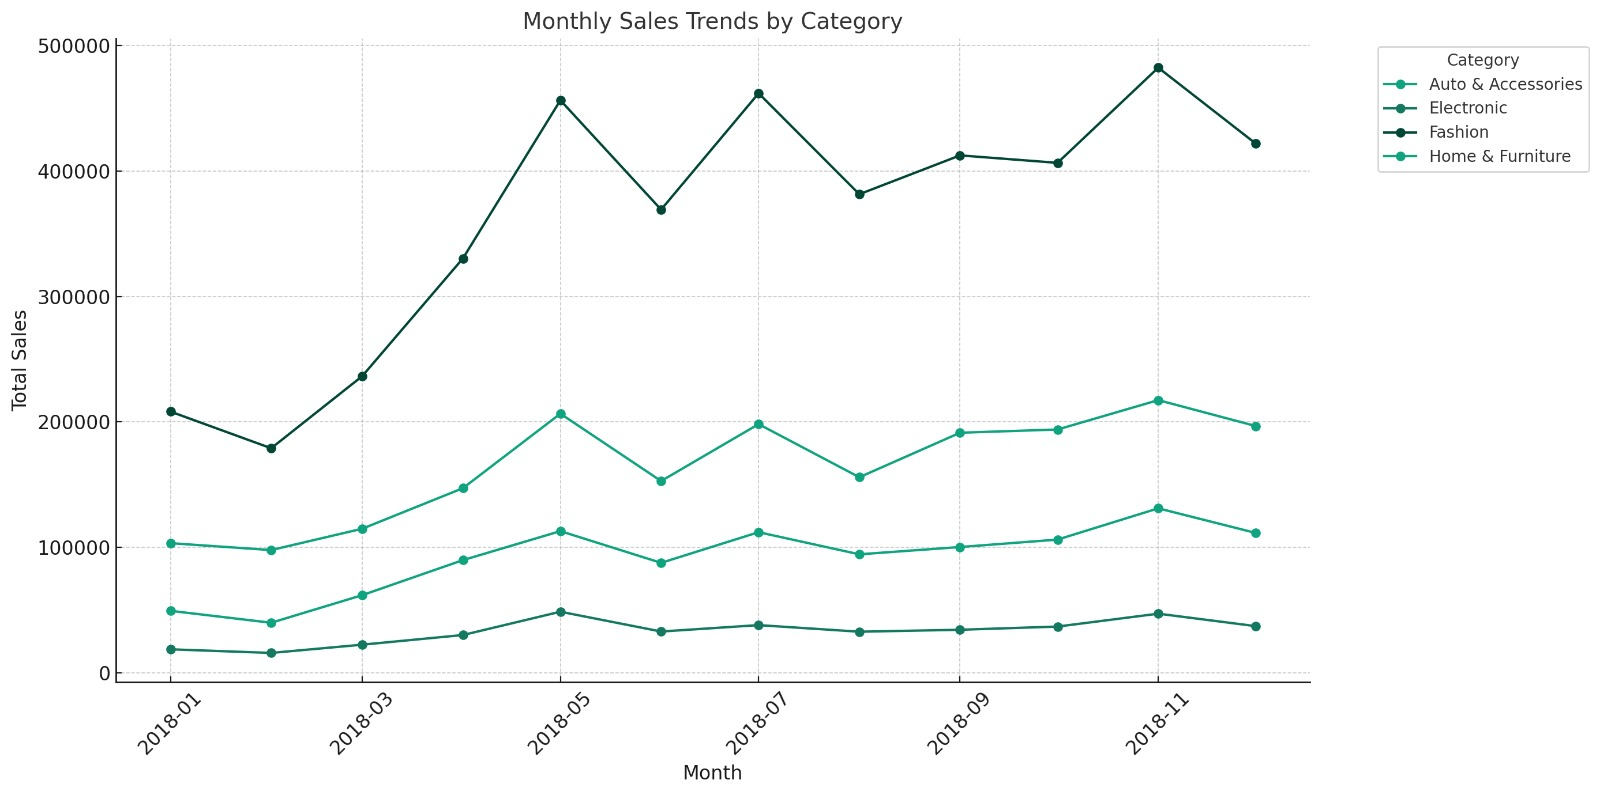
\includegraphics[width=0.5\textwidth]{goal1.jpeg}
\end{itemize}



\subsection{Goal 2: Sales Performance by Gender}
\begin{lstlisting}[language=Python, caption={Sales performance analysis by gender}]
gender_sales_performance = df.groupBy("Gender").sum("Sales")
                             .orderBy("Total_Sales")
gender_sales_performance.show()
\end{lstlisting}
\subsubsection{Results}
The sales performance analysis by gender provided the following findings:

\begin{itemize}
    \item (Insert insights or observations about sales performance by gender)
     \item \textbf{Visualization}: 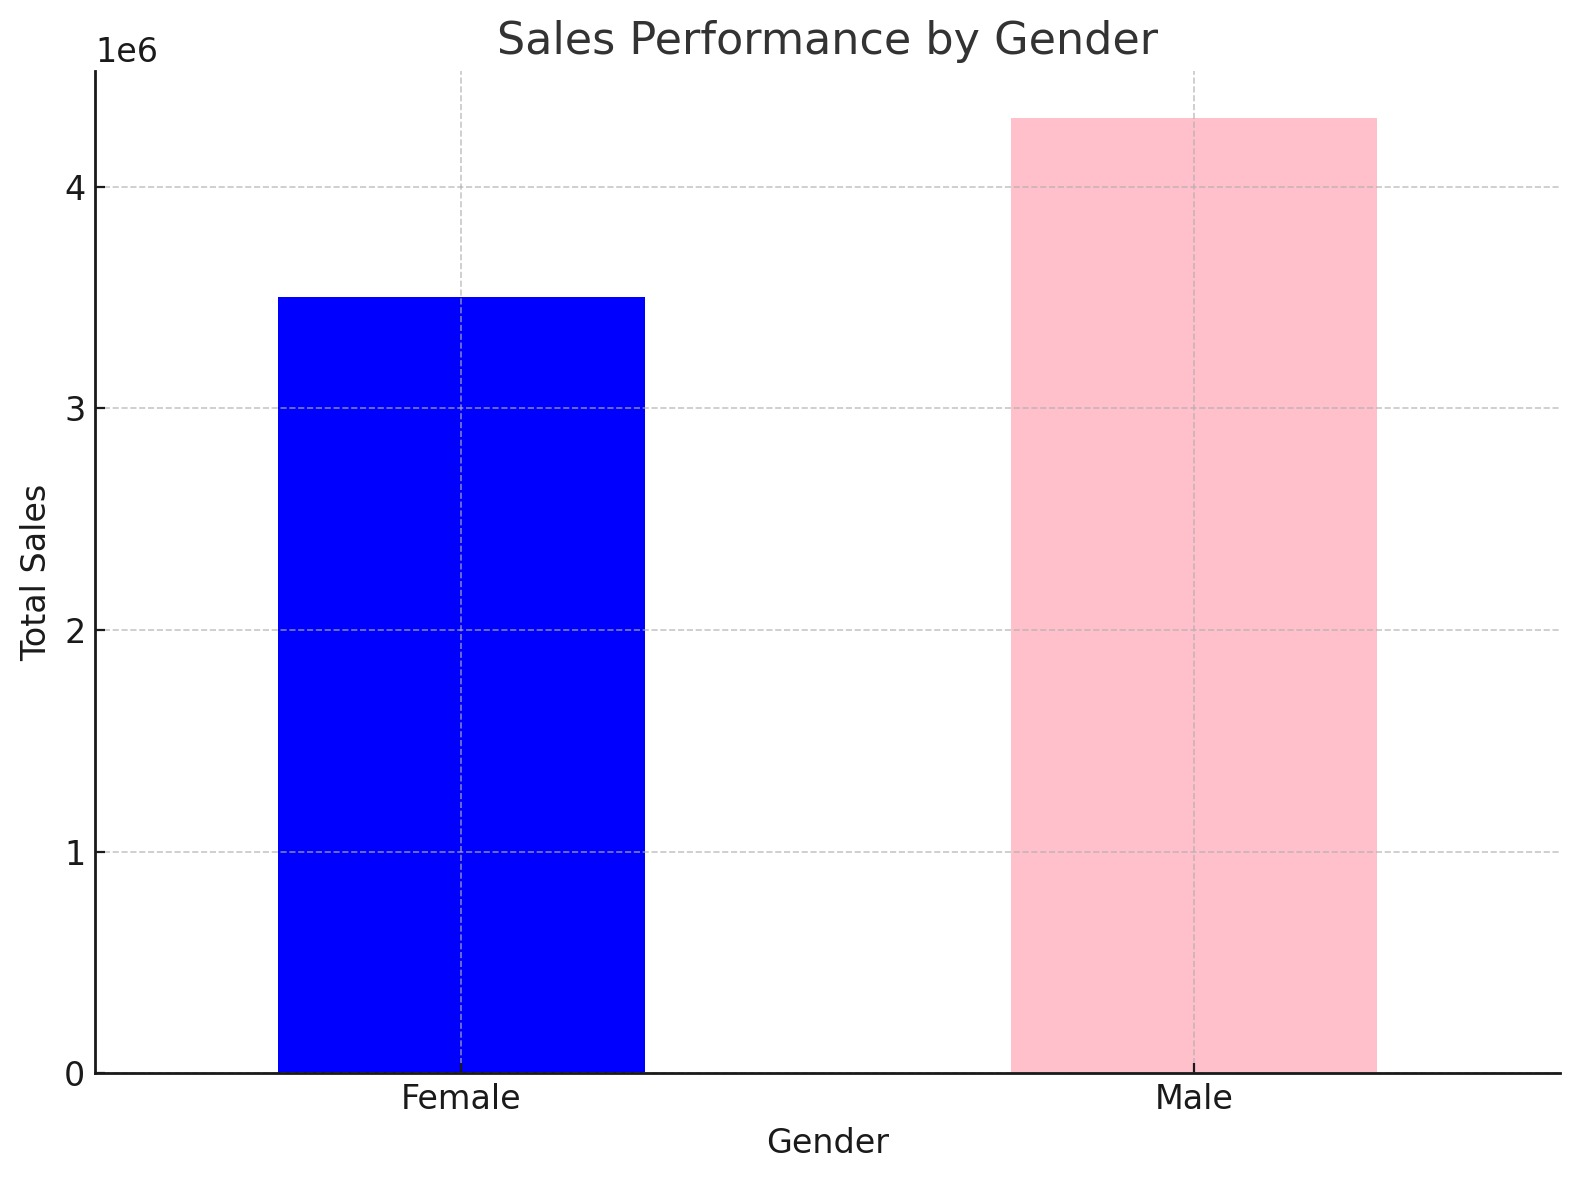
\includegraphics[width=0.5\textwidth]{goal2.jpeg}
\end{itemize}

% Repeat the above structure for the remaining goals...

\subsection{Goal 3: Effectiveness of Discount Strategies}
\begin{lstlisting}[language=Python, caption={Analyzing the effectiveness of discount strategies}]
discount_sales_effectiveness = df.groupBy("Discount").sum("Quantity")
                                 .orderBy("Discount")
discount_sales_effectiveness.show()
\end{lstlisting}
\subsubsection{Results}
The analysis of discount strategies revealed:

\begin{itemize}
    \item (Insert insights or observations about the effectiveness of discount strategies)
    \item \textbf{Visualization}: 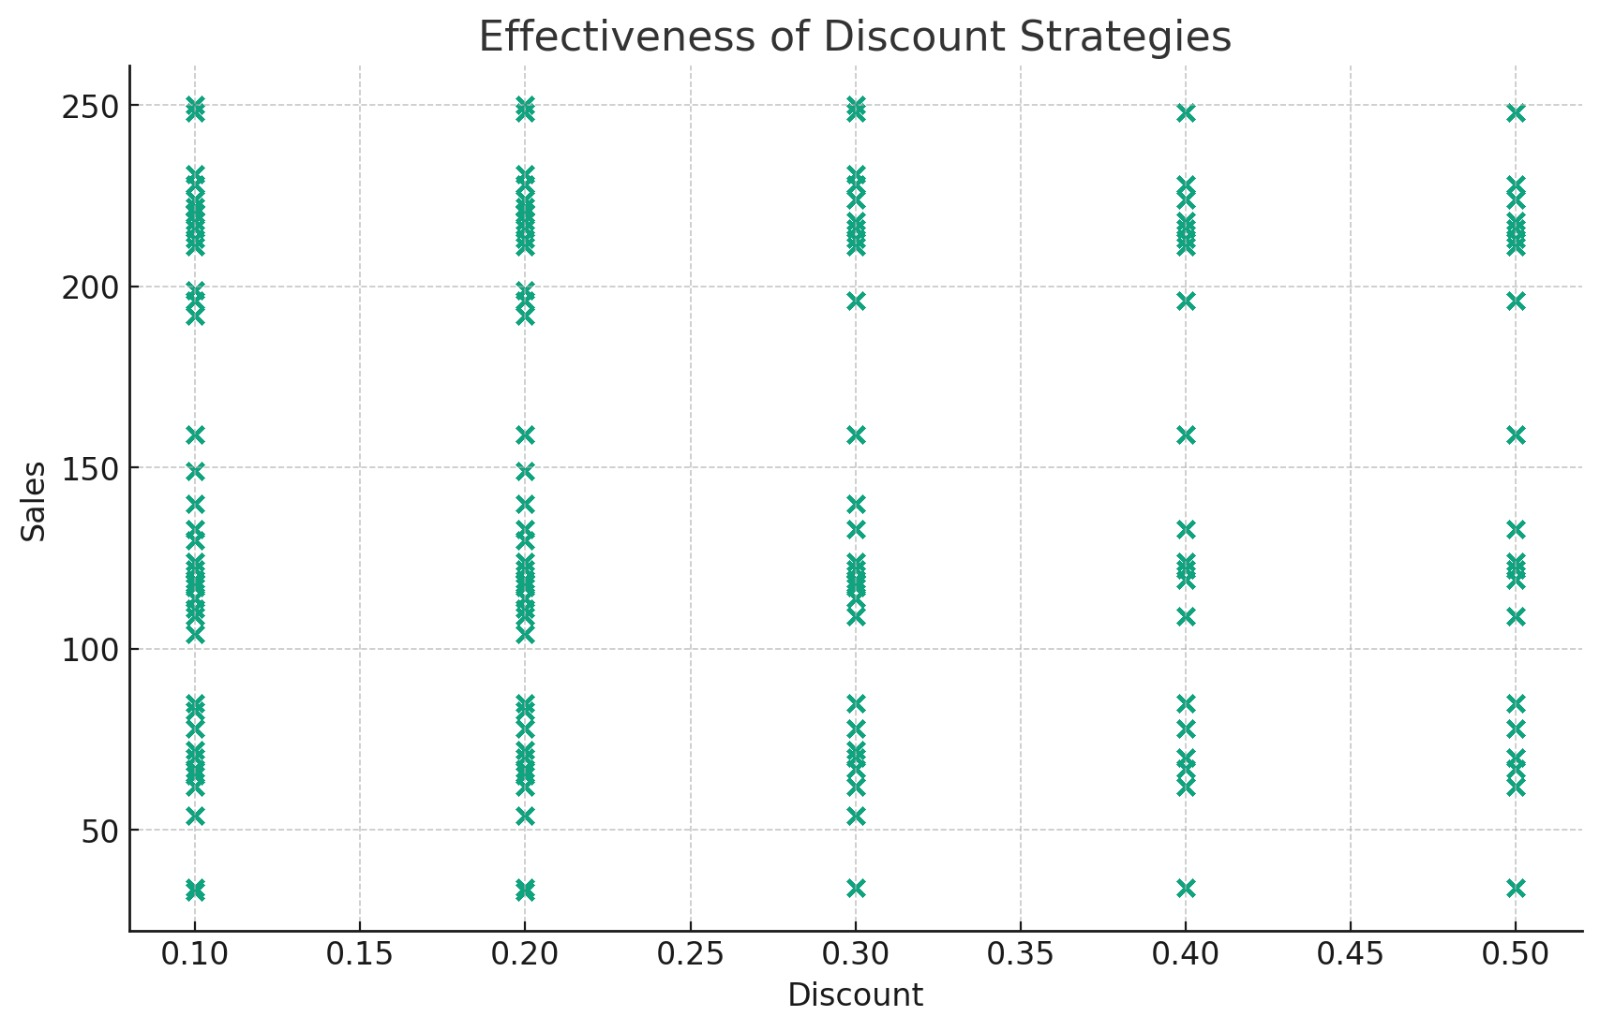
\includegraphics[width=0.5\textwidth]{goal3.jpeg}
\end{itemize}

\subsection{Goal 4: Profit Analysis by Product}
\begin{lstlisting}[language=Python, caption={Profit analysis per product}]
product_profit_analysis = df.groupBy("Product").sum("Profit")
                            .orderBy("Total_Profit", ascending=False)
product_profit_analysis.show()
\end{lstlisting}
\subsubsection{Results}
The profit analysis by product showed:

\begin{itemize}
    \item (Insert insights or observations about profit analysis per product)
     \item \textbf{Visualization}: 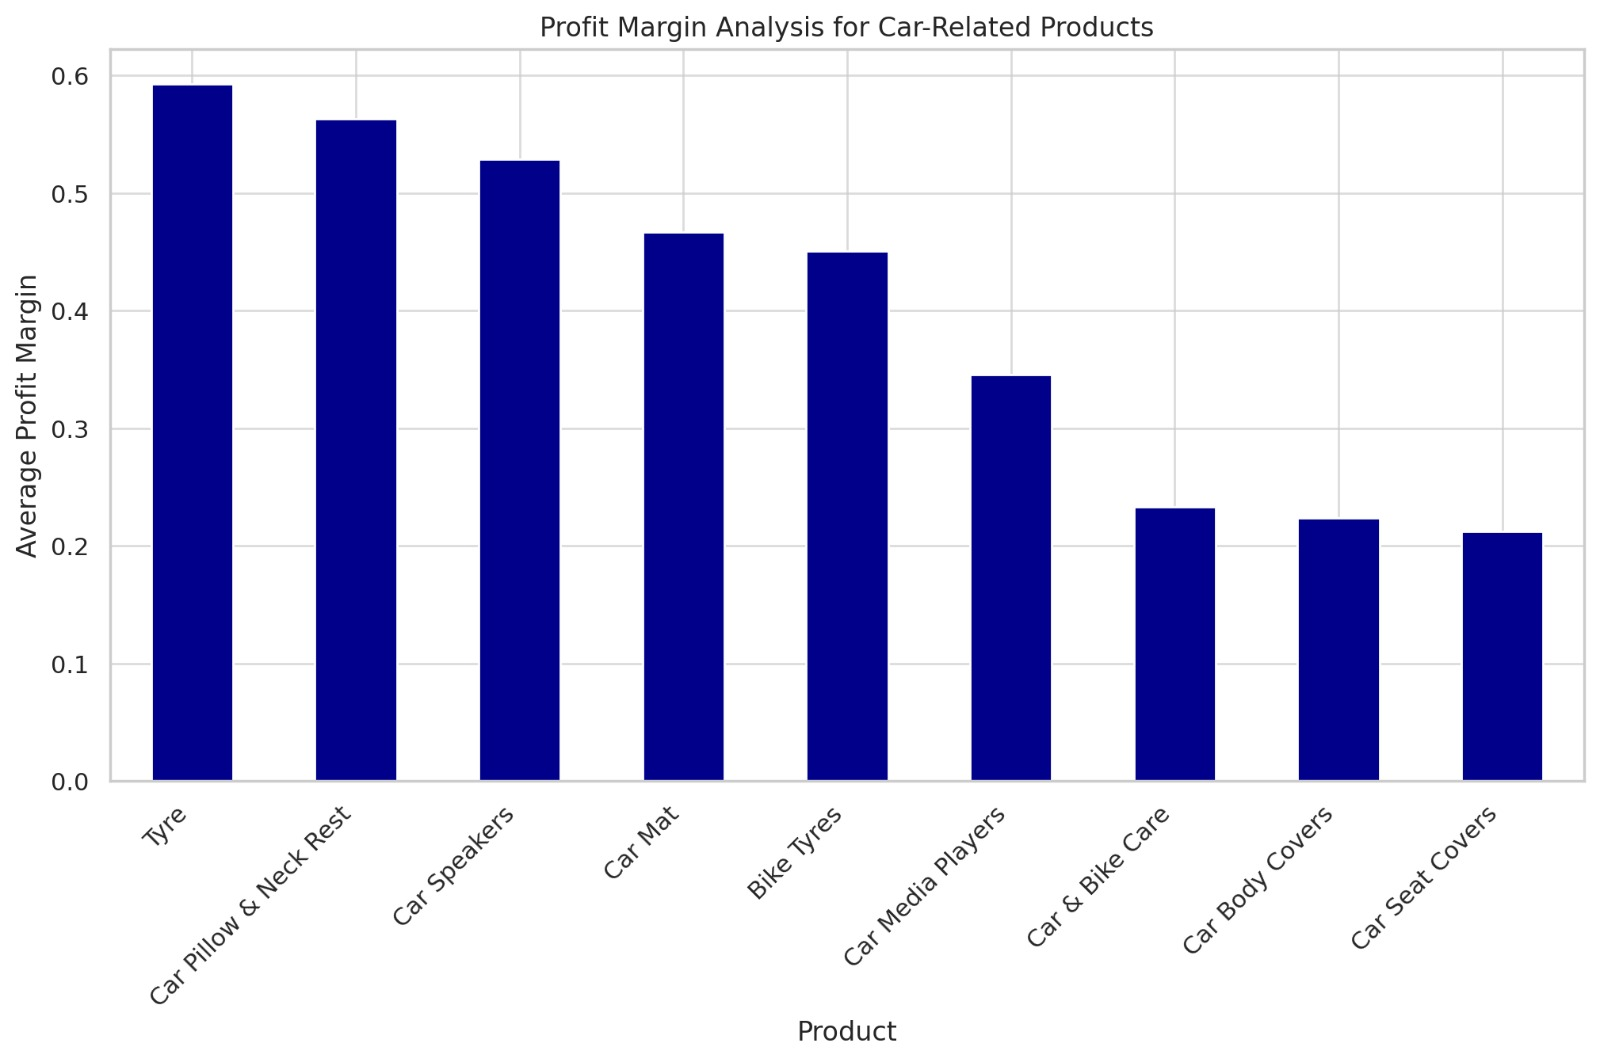
\includegraphics[width=0.5\textwidth]{goal4.jpeg}
\end{itemize}
\subsection{Goal 5: Customer Retention Analysis}
\begin{lstlisting}[language=Python, caption={Customer retention analysis}]
customer_retention = df.groupBy("Customer_Id")
                       .agg(countDistinct("Order_Date"))
                       .orderBy("Unique_Purchase_Dates", ascending=False)
customer_retention.show()
\end{lstlisting}
\subsubsection{Results}
The customer retention analysis indicated:

\begin{itemize}
    \item (Insert insights or observations about customer retention)
     \item \textbf{Visualization}: 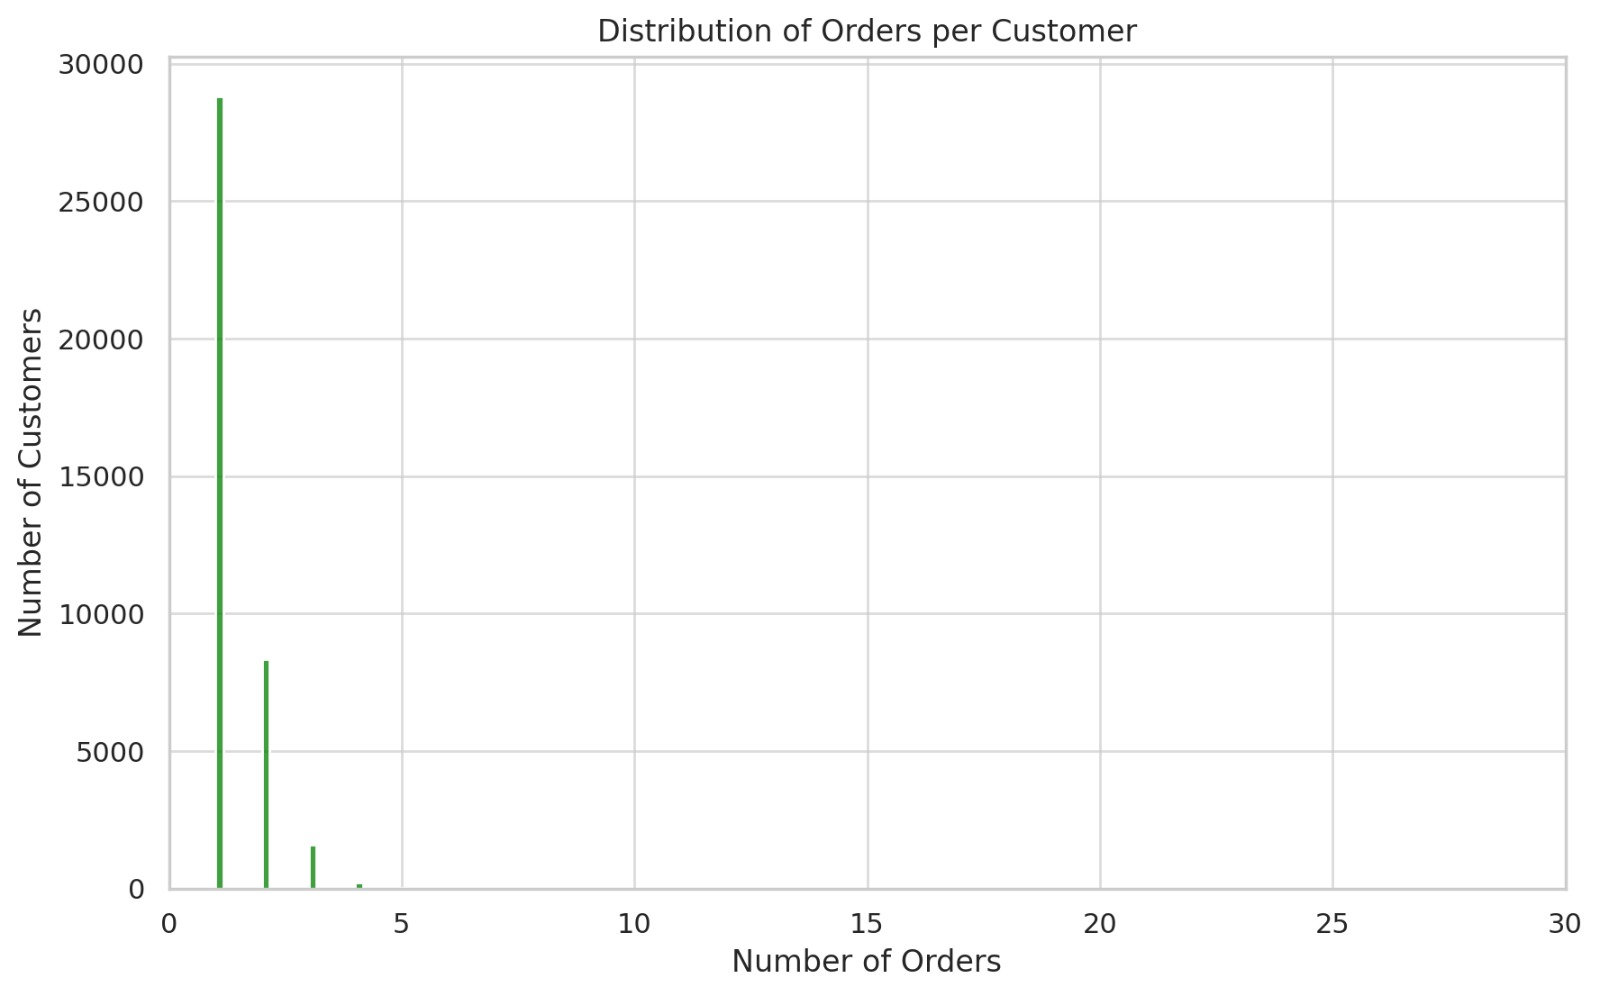
\includegraphics[width=0.5\textwidth]{goal5.jpeg}
\end{itemize}

\subsection{Goal 6: Payment Method Preferences}
\begin{lstlisting}[language=Python, caption={Payment method usage analysis}]
payment_method_usage = df.groupBy("Payment_method").count()
                         .orderBy("Usage_Count", ascending=False)
payment_method_usage.show()
\end{lstlisting}
\subsubsection{Results}
The analysis of payment method preferences revealed:

\begin{itemize}
    \item (Insert insights or observations about payment method usage)
     \item \textbf{Visualization}: 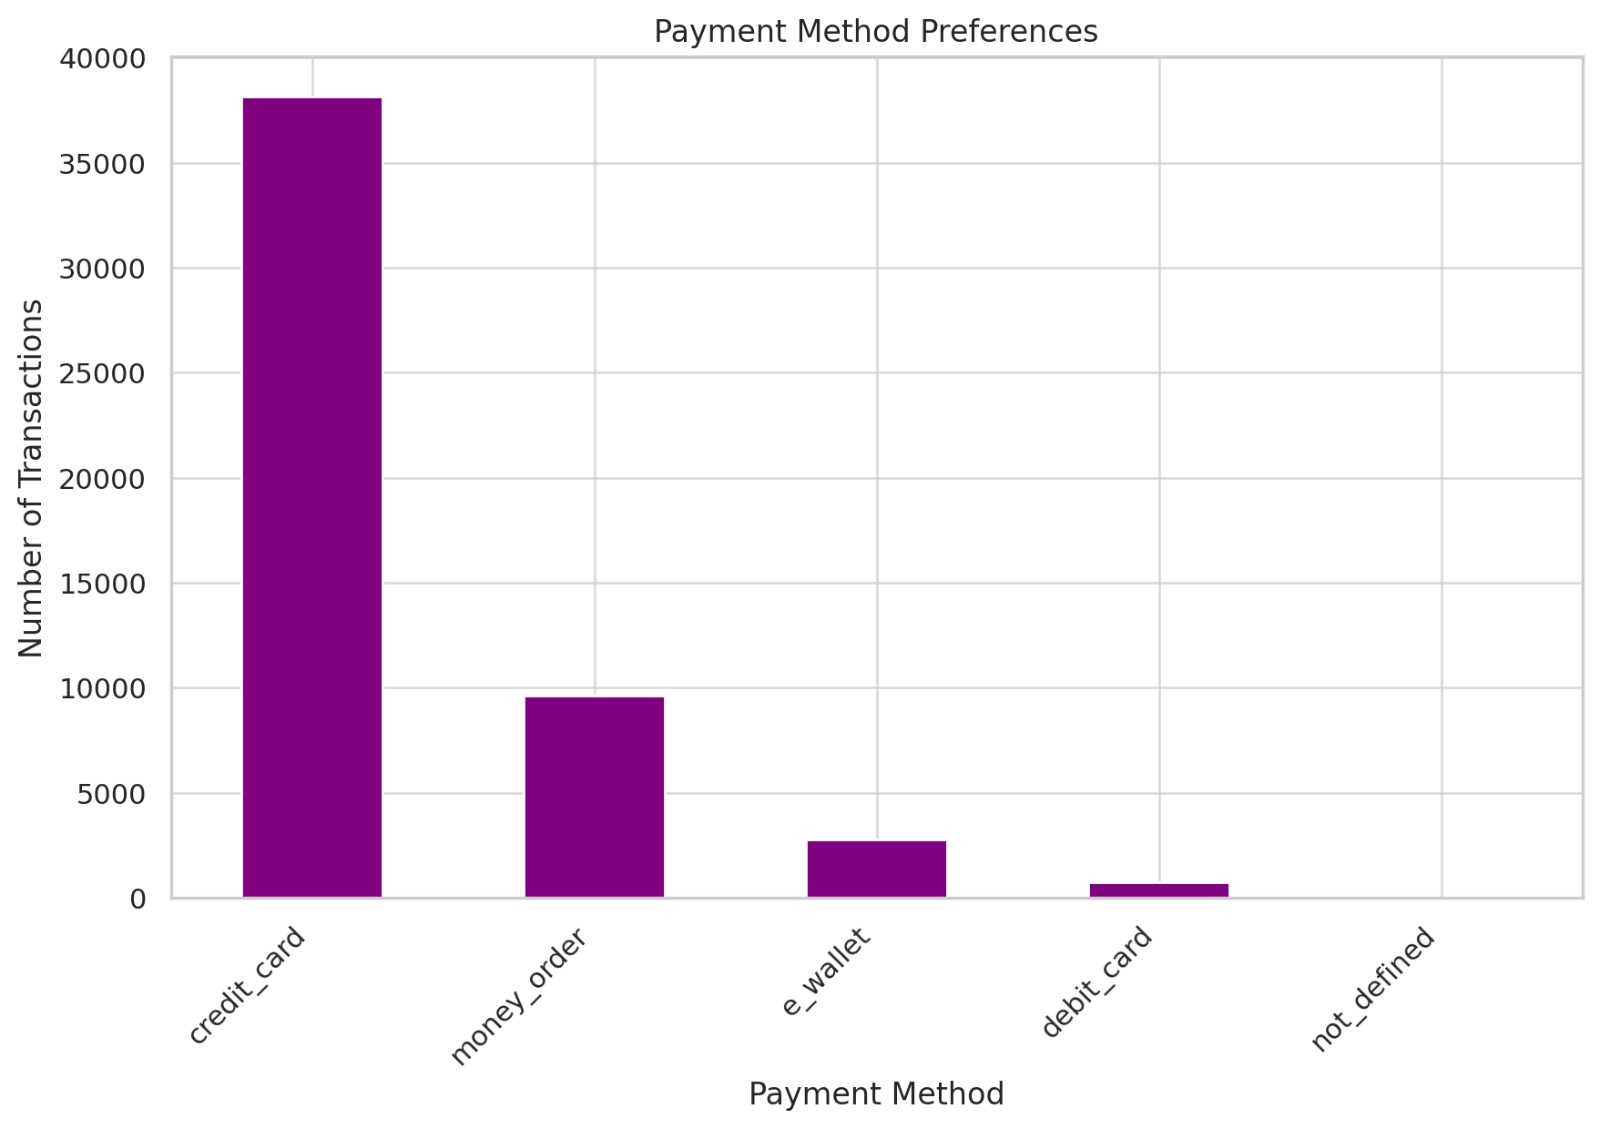
\includegraphics[width=0.5\textwidth]{goal6.jpeg}
\end{itemize}

\subsection{Goal 7: Shipping Cost Analysis}
\begin{lstlisting}[language=Python, caption={Shipping cost impact analysis}]
shipping_cost_impact = df.groupBy("Shipping_Cost").sum("Sales")
                         .orderBy("Shipping_Cost")
shipping_cost_impact.show()
\end{lstlisting}
\subsubsection{Results}
The shipping cost analysis indicated:

\begin{itemize}
    \item (Insert insights or observations about shipping cost impact)
    \item \textbf{Visualization}: 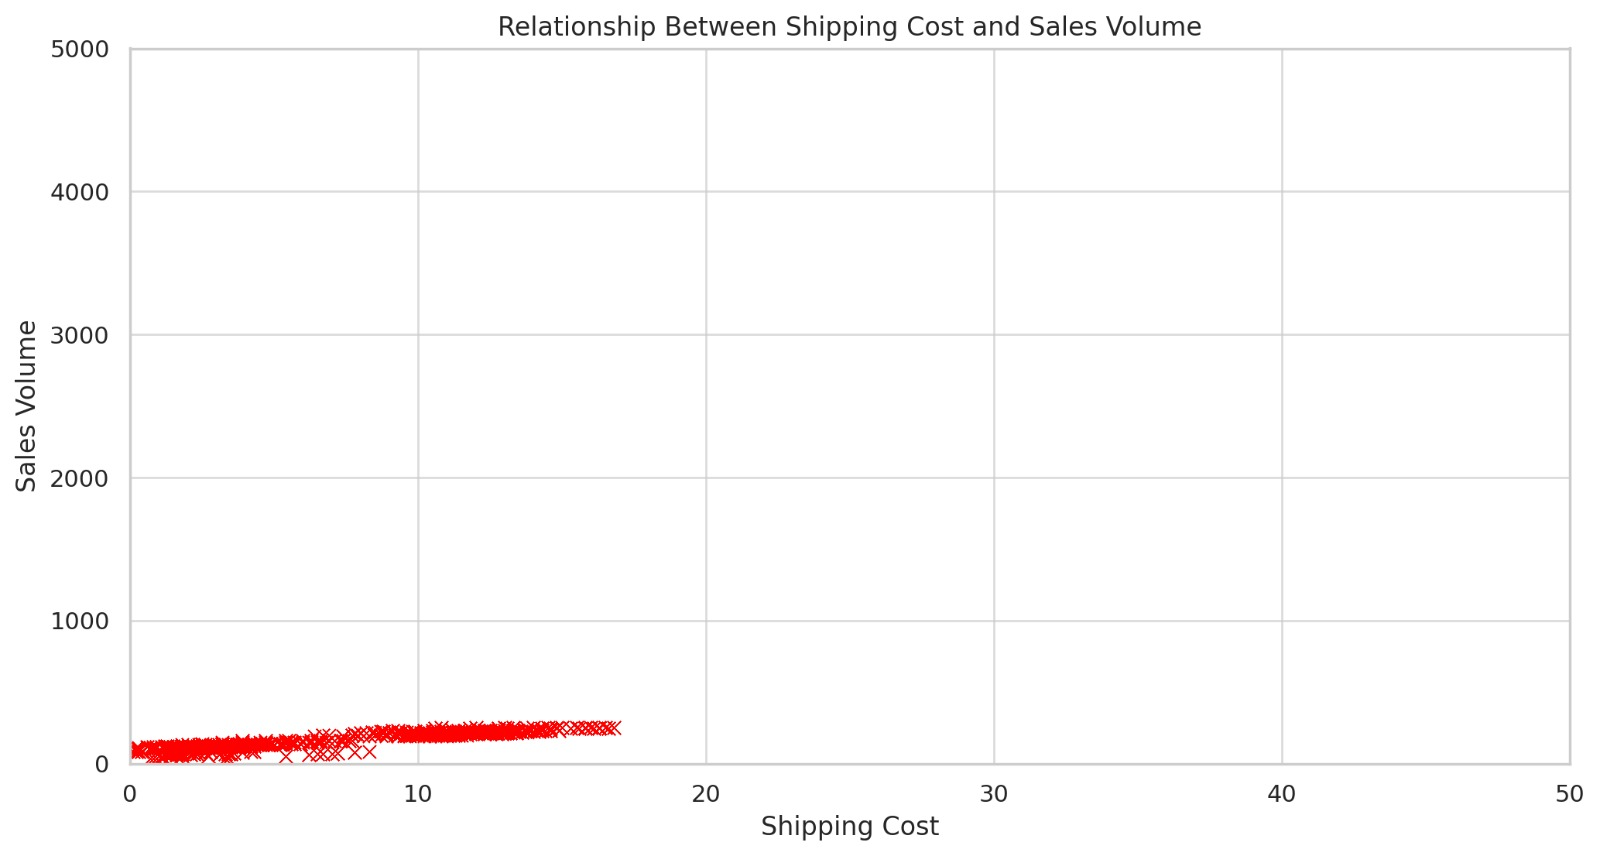
\includegraphics[width=0.5\textwidth]{goal7.jpeg}
\end{itemize}

\subsection{Goal 8: Order Priority Effect on Sales Volume}
\begin{lstlisting}[language=Python, caption={Order priority and its effect on sales volume}]
order_priority_sales = df.groupBy("Order_Priority").sum("Quantity")
                         .orderBy("Order_Priority")
order_priority_sales.show()
\end{lstlisting}
\subsubsection{Results}
The analysis of order priority on sales volume showed:

\begin{itemize}
    \item (Insert insights or observations about order priority's effect on sales volume)
    \item \textbf{Visualization}: 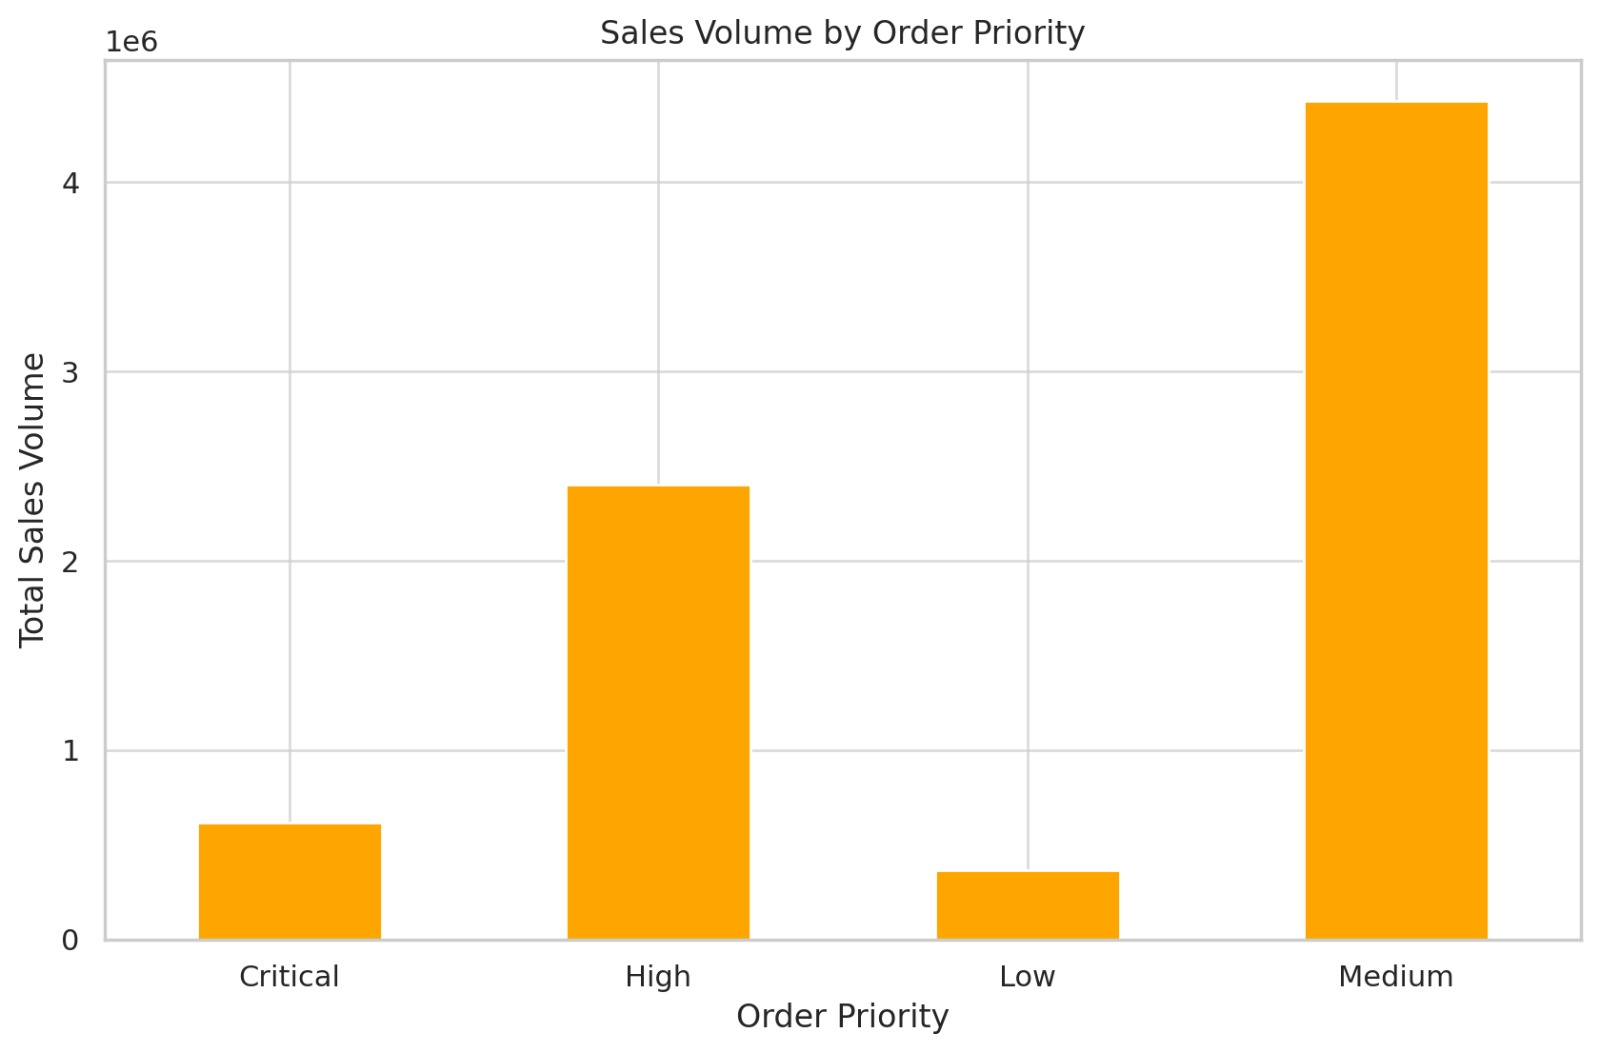
\includegraphics[width=0.5\textwidth]{goal8.jpeg}
\end{itemize}
\section{Conclusion}
This document presented a detailed approach for analyzing E-commerce data to discover retail trends using Map-Reduce operations. The goals were carefully chosen to address various facets of the retail industry and were successfully implemented using PySpark.

\section{References}
All references to external resources and documentation used will be listed here.

\section{GitHub Repository}
The complete source code and documentation for the project can be found at:
\href{https://github.com/RoshiniNwmsu/The-Sparkling-Analysts}{https://github.com/RoshiniNwmsu/The-Sparkling-Analysts}

\end{document}